\chapter{Implementation}
% Introducing the Chapter
This chapter gives an overview of the developed musical multi-robot system. The main goal of the implemented system is to allow for individual musical agents in a musical multi-agent collective to interact with each other, in order to achieve emergent and co-ordinating behaviour—in our case synchronization—with varying degrees of self-awareness, collective-sizes, and of difficulty and certainty in the environment and communication. More specifically, the goal with the design is to enable the robot collective to achieve so-called \textit{harmonic synchronization} within a relatively short time. Exactly what is meant by \textit{harmonic synchronization} will be expounded in Section \ref{sec:harmonic_synchrony}.

These goals firstly require of the agents the modelling of oscillators with their properties, like phase and frequency, as explained further in Subsection \ref{subsec:agent}. To allow for interaction and communication between the agents, mechanisms so that the agents can transmit "fire"-signals, as well as listen for other agents's "fire"-signals, is necessary as well, and is presented in Subsection \ref{subsec:fire_signal}.

First, the system and the system components will be presented and introduced. Then, methods implemented for achieving the system target goal of \textit{harmonic synchrony} in various synchronization objectives—firstly solely for oscillator-phases, then secondly for both oscillator-phases and oscillator-frequencies—will be described and presented.

A helpful way to read this chapter could be as answers to the question "how can one achieve and detect the final part of the chapter by performing the middle part to the first one?" — more specifically "how can one achieve and detect the target/goal state of harmonic synchrony, by performing updates to the musical robots's phases and frequencies, in the musical multi-robot collective?"




% SECTION 1, Introducing the System and the System-components:
\section{The musical multi-robot collective}
\label{sec:developed_system}

	Envision that we have a multi-agent collective scenario consisting of musical robots modelled as oscillators, solely communicating through brief ``fire''-like audio-signals—greatly inspired by K. Nymoen et al.'s synchronizing ``fireflies'' \cite{nymoen_synch}. These agents are not initially synchronized in their firing of audio-signals; but as time goes, they are entraining to synchronize to each other by adjusting their phases and frequencies when/after hearing each other's audio-/fire-signals. If they then, after some time of listening and adjusting, succeed in becoming synchronized — we then will eventually see ``fire''-events/-signals line up at an even underlying pulse or rhythm. Examples and demonstrations of this process are depicted in Figure \ref{fig:first_idea:first_fig} and \ref{fig:first_idea:second_fig}.

	% First Intro-illustration figure to easily get a quick idea of what the system/design does/consists of (to be exchanged with a describing system scheme/diagram):
	\begin{figure}[h]
	\centering
	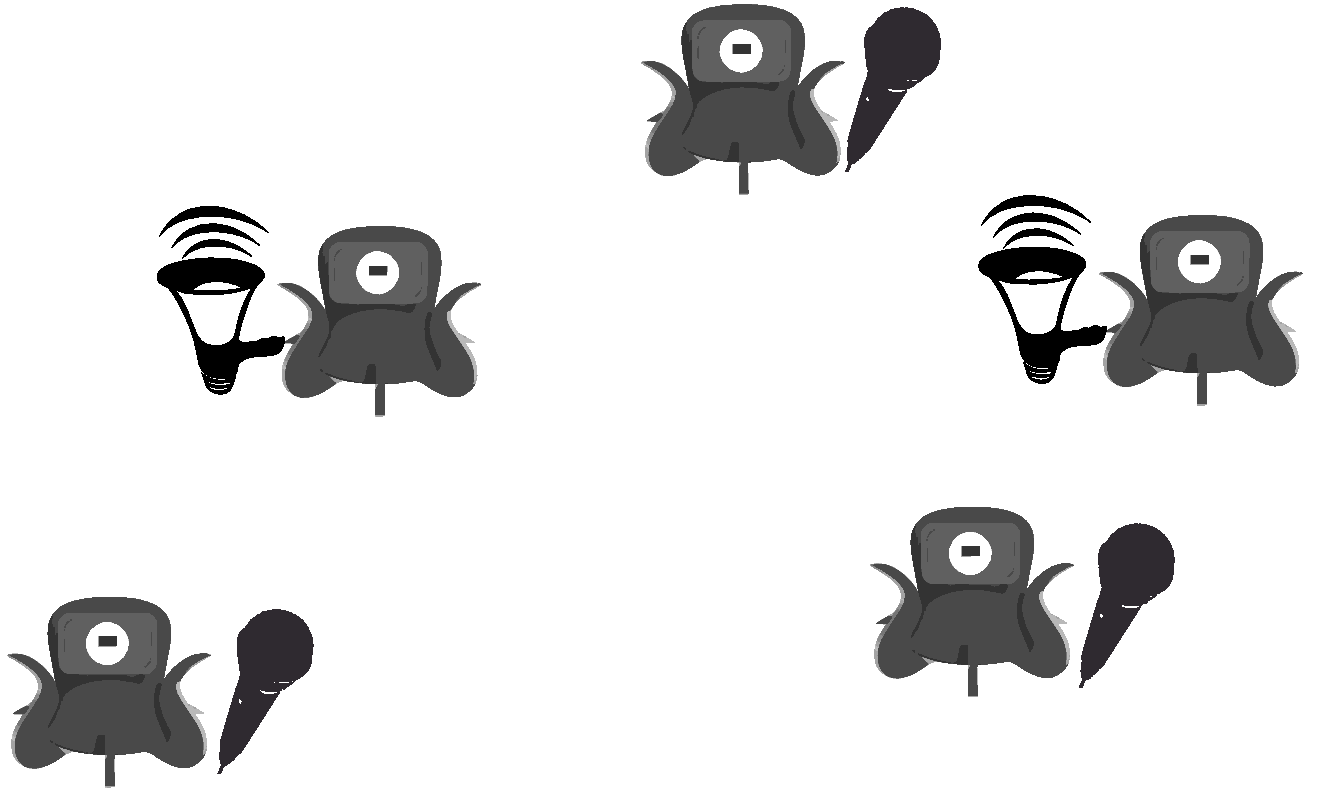
\includegraphics[width=0.9\linewidth]{Assets/Figures/schematic_initial_idea.pdf}
	\caption{Illustration/Schematic: Musical robot collective moving towards achieving harmonic synchronization, through performing phase- \& frequency-adjustments. Agents that are not firing at the moment will adjust themselves after hearing a ``fire''-/adjustment-signal from a neighbouring firing agent.}
	\label{fig:first_idea:first_fig}
	\end{figure}

	% Second Intro-illustration figure to easily get a quick idea of what the system/design does/consists of (to be exchanged with a describing system scheme/diagram):
	\begin{figure}[ht!]
		\centering
			\begin{subfigure}[t]{.5\textwidth}
				\centering\captionsetup{width=.9\linewidth}%
				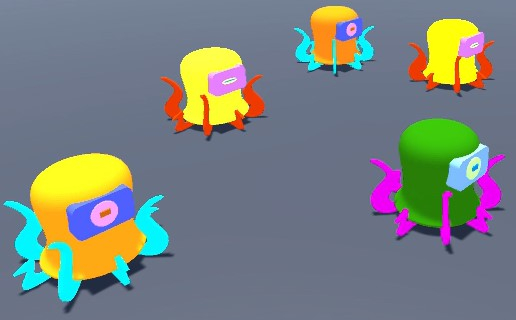
\includegraphics[width=0.9\linewidth]{Assets/Figures/IntroUnsynch.jpg}
				\caption{Agents firing, i.e. blinking with their eyes and turning their body yellow, asynchronously at first. Only two Dr. Squiggles-robots with red tentacles fire simultaneously, the rest do not.}
				\label{fig:first_idea:second_fig:unsynched}
			\end{subfigure}%
			\begin{subfigure}[t]{.5\textwidth}
				\centering\captionsetup{width=.9\linewidth}%
				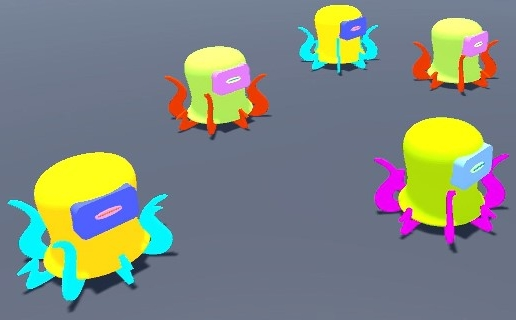
\includegraphics[width=0.9\linewidth]{Assets/Figures/IntroSynch.jpg}
				\caption{Seconds later, after having listened to each others's adjustment-signals and adjusted themselves accordingly, all agents are here firing simultaneously and synchronously.}
				\label{fig:first_idea:second_fig:synched}
			\end{subfigure}
		\caption{From simulation: Example of harmonic synchronization achieved in a musical robot collective, where frequencies are equal and constant, but phases are heterogenous and randomly initialized. This is the first and simpler problem to solve, synchronizing the phases $\phi_i$ for all agents $i$, which we will refer to as \textit{the $\phi$-problem}. The second and harder problem of synchronizing both phases $\phi_i$, as well as frequencies $\omega_i$, we will refer to as \textit{the $\phi$- \& $\omega$-problem}.}
		\label{fig:first_idea:second_fig}
	\end{figure}

	% INCLUDE PHASES UNSYNCHED VS. SYNCHED PLOT? See 'Relevant MSc-thesis Concerns'.
		% % Phase-/time-plot Figure with two Subplots. Subplot 1: phase-/time-plot when oscillators are unsynchronized. Subplot 2: phase-/time-plot when oscillators are synchronized
		% \begin{figure}[h]
			% \centering
				% \begin{subfigure}[t]{.5\textwidth}
					% \centering\captionsetup{width=.9\linewidth}%
					% 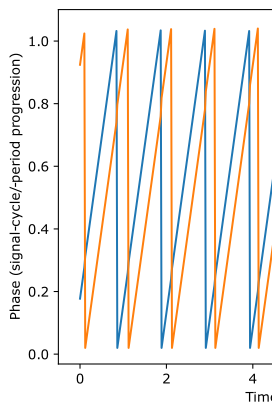
\includegraphics[width=0.9\linewidth]{Assets/Figures/phases_unsynched.png}
					% \caption{Oscillators are initially not (phase-) synchronized.}
					% \label{fig:phases_unsynched}
				% \end{subfigure}%
				% \begin{subfigure}[t]{.5\textwidth}
					% \centering\captionsetup{width=.9\linewidth}%
					% 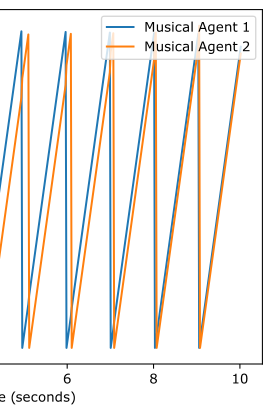
\includegraphics[width=0.9\linewidth]{Assets/Figures/phases_synched.png}
					% \caption{Oscillators are now, seconds later, (phase-) synchronized.}
					% \label{fig:phases_synched}
				% \end{subfigure}
			% \caption{Phase-plots for the agents}
			% \label{fig:initial}
		% \end{figure}




	% Introducing the System Components:
	
	% Om den enkelte noden/agenten med alle egenskaper den har osv.
	\subsection{The individual agent: a musical robot}
	\label{subsec:agent}
		The musical robot collective consists of M. J. Krzyzaniak and RITMO's musical robots, the Dr. Squiggles. \nl
		
		Om hver individuelle agents egenskaper og karakteristikker.
		
		Hver individuelle agent består av noen deler:
		\begin{itemize}
			\item For eksempel en oscillator-komponent.
			\item Noe inspirert fra I.A, III.Intro., og 'Implementation' i Nymoen's firefly-paper
		\end{itemize}
		
		(as e.g. an oscillator-component (cf. I.A, III.Intro., and 'Implementation' in Nymoen's firefly-paper))
		
		All agents have the ability to listen for transmitted ``fire''-signals from their neighbours, which they then will use as a trigger to adjust themselves according to some well-designed update-functions to be elaborated upon in Section \ref{sec:phase_methods} and \ref{sec:frequency_methods}.

		Notions like ``agent'', ``robot'', ``firefly'', and ``oscillator'' will be used interchangeably throughout the thesis.



	% Om kommunikasjonen til agentene: audio-/``fire''-signalet
	\subsection{Robot communication: the ``fire''-signal}
	\label{subsec:fire_signal}
	
	These aforementioned audio-signals, also referred to as ``fire''-signals, are transmitted whenever an agent's oscillator \textit{peaks} (i.e. after its cycle or period is finished, having phase $\phi(t)=1$) — or actually every second \textit{peak} due to the system target goal of \textit{harmonic synchrony}
, to be elaborated upon in Section \ref{sec:harmonic_synchrony}.

	Hva er signalene, hvordan ser de ut (kanskje diskutere simulering vs. virkeligheten), og hvordan sendes de ut? Hva skjer når de blir sendt ut?
	
		\begin{itemize}
			\item Short and impulsive audio sound/signal, representing an agent's phase-climax and ``fire''-/``flash''-event.
			\item Stigmergic co-ordination/communication.
			\item Facilitating PCO (pulse-coupled oscillators), different from phase-coupled oscillators with their differences.
			\item Aspekter fra Nymoens paper som presentert i Essay-oppsummeringen min.
		\end{itemize}
	
	No individual agent is able to adjust or modify the state of any other agent, only its own, and the only means of communication between the agents will be through these ``fire''-signals.
	
	
	
	
	
	
	
	
	
	




% SECTION 2, Presenting Methods for Phase-Adjustment:
\section{Synchronizing oscillator-phases}
\label{sec:phase_methods}

	If we first assume constant and equal oscillator-frequencies in our agents, we can take a look at how the agents adjust their|initially random|phases in order to synchronize to each other. This is then in contrast to the case in Section \ref{sec:frequency_methods} where heterogenous and randomly initialized oscillator-frequencies in the musical agents are used and synchronized.
	
	The goal state of the agents is for now to fire/flash simultaneously, after having started firing/flashing at random initially. Note that this is a special case of the final and ultimate goal of \textit{harmonic synchrony}. This is due to how all agents in the collective firing/flashing simultaneously, is considered having achieved harmonic synchrony since its phases would be synchronized if fire-events are lined up in even pulses, as well as all frequencies in the agent collective being within the set of ``legal'' frequencies, $\omega_{0} \cdot 2^{\mathbb{N}_0}$, where $\omega_0$ is the fundamental (smallest) frequency in the agent collective, and $0 \in \mathbb{N}_0$ — leading to $\omega_0 \cdot 2^0 = \omega_0$ to be a legal frequency, which is what all agents in our case here have as frequences.
	
	In order for the musical agents to synchronize to each other, they will have to—due to their heterogenous and randomly initialized phases—adjust or update their own phases according to some well-designed update-/adjustment-functions, as presented below.
	
	When it comes to the temporality and timing of when these updating functions are used and applied; Musical agents's phases get updated/adjusted immediately as ``fire''-/``flash''-events from neighbouring robots are perceived.

	
	
	% Mirollo-Strogatz's Phase-Adjustment
	\subsection{Mirollo-Strogatz's ``standard'' phase-adjustment} % used '-adjustment' before
	
	One approach having been used to achieve this in the past is Mirollo-Strogatz's ``Standard'' Phase-adjustment in oscillators \cite{mirollo_strogatz_PCO_synch}, as illustrated in Figure \ref{fig:strog_phase}.
			
	\begin{figure}[h]
		\centering
		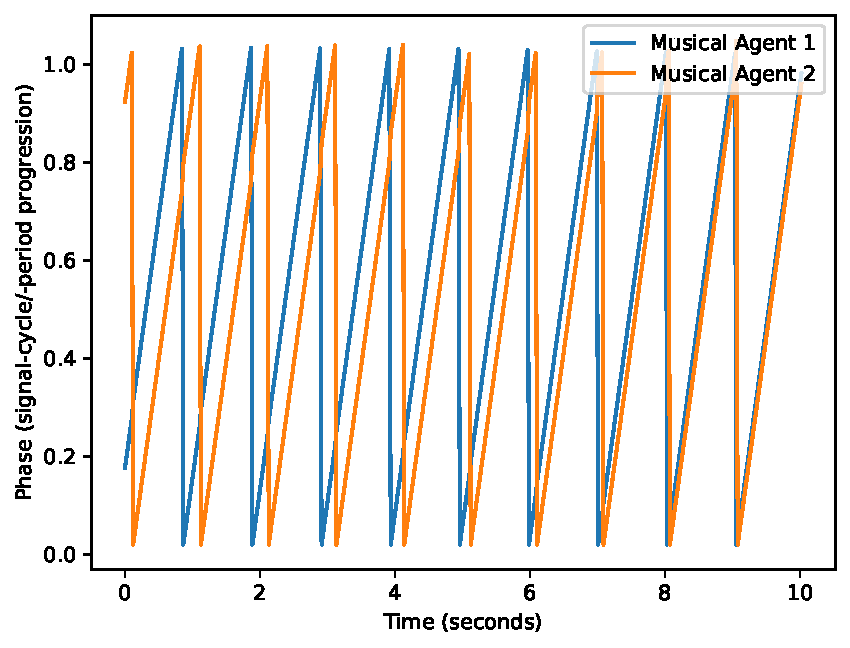
\includegraphics[width=0.9\linewidth]{Assets/Figures/MirolloStrogatzPhaseAdjustment.pdf}
		\caption{``Standard'' phase-adjustment with Mirrollo-Strogatz's approach}
		\label{fig:strog_phase}
	\end{figure}
	
	Each musical agent gets a new phase, $\phi(t^+) = P(\phi(t))$, accoring to the \textbf{phase update function \eqref{strog_phase}} upon perceiving a ``fire''-event from one of the other musical nodes:
	
	\begin{equation}\label{strog_phase}
	P(\phi(t)) = (1 + \alpha)\phi(t)	,
	\end{equation}
	
	where ``\textit{$\alpha$ is the pulse coupling constant, denoting the strength between nodes}'' \cite{nymoen_synch}, and $t^+$ denotes the time-step immediately after phase-climax. So, if $\alpha = 0.1$ e.g., then a musical agent's new and updated phase, immediately after hearing a ``fire''-signal from another agent, will be equal to $\phi(t^+) = P(\phi) = (1 + 0.1)\phi = 1.1\phi$. 110\% of its old phase $\phi$, that is. Hence, and in this way, the agent would be ``pushed'' to fire sooner than it would otherwise (as nodes fire once they have reached phase-climax $\phi=1$).
		
	
	
	
	% K. Nymoen's Phase-Adjustment
	\subsection{K. Nymoen's bi-directional phase-adjustment} % used 'Shifts' before
	
	\begin{figure}[h]
		\centering
		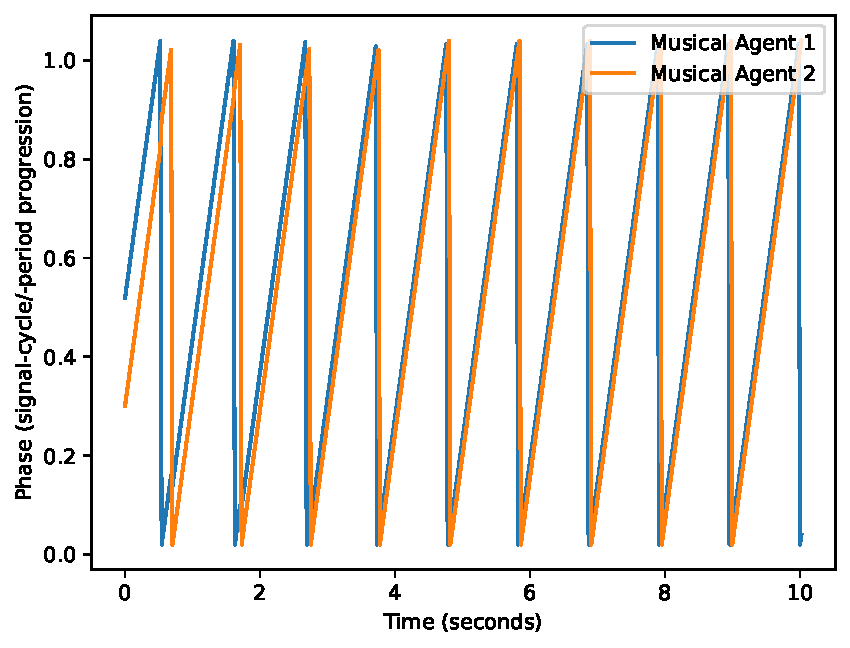
\includegraphics[width=0.9\linewidth]{Assets/Figures/NymoenPhaseAdjustment.pdf}
		\caption{Bi-directional phase-adjustment with K. Nymoen et al.'s approach}
		\label{fig:nymoen_phase}
	\end{figure}
	
	This phase-adjustment, as in Figure \ref{fig:nymoen_phase}, works very similarly to the phase-adjustment performed in the ``standard'' \textbf{\textit{Mirollo-Strogatz}} approach presented earlier; the only difference being that now, nodes update their phases with the slightly more complex \textbf{phase update function \eqref{nymoen_phase}} when hearing a ``fire''-event from one of the other musical nodes — allowing for both larger, but also smaller, updated phases compared to the old phases:
	
	\begin{equation}
	\label{nymoen_phase}
		P(\phi) = \phi - \alpha \cdot sin(2\pi\phi) \cdot | sin(2\pi\phi) |
	\end{equation}
	
	The fact that new and updated phases can both be larger, but also smaller, compared to the old phases, is exactly what's meant by the Phase-adjustment being \textbf{\textit{bi-directional}}, or as the authors call it in the paper as using ``\textit{both excitatory and inhibitory phase couplings between oscillators}'' \cite{nymoen_synch}.
	
	The effects then of adjusting phases—upon hearing ``fire''-events, according to this newest update-function \eqref{nymoen_phase}—are that the nodes's phases now get decreased if $\phi(t)$ is lower than 0.5, increased if $\phi(t)$ is higher than 0.5, and neither—at least almost—if the phases are close to $0.5$. This is due to the negative and positive sign of the sinewave-component in Equation \eqref{nymoen_phase}, as well as the last attenuating factor in it of $| sin(2\pi\phi) | \approx | sin(2\pi \frac{1}{2}) | = | sin(\pi) | = | 0 | = 0$, then if we have $\phi(t) \approx 0.5 = \frac{1}{2}$.

	
	
	
	
	
	










	

% SECTION 3, Presenting Methods for Frequency-Synchronization:
\section{Synchronizing oscillator-frequencies}
\label{sec:frequency_methods}

	% Om Update-functions for frekvens-oppdateringene
	Now over to the slightly more complex issue of adjusting and synchronizing frequencies in the agent-/oscillator-collective. We introduce randomly initialized, non-constant, and heterogenous oscillator-frequencies in our musical agents — allowing in the music collective the playing of diverse rhythmic patterns. The agents are now required to synchronize their initially different and random frequencies, so that frequencies are ``legal'' and \textit{harmonically synchronized}. Such ``legal'' frequencies are described clearly in detail in Section \ref{sec:harmonic_synchrony}.
	
	In order for the musical agents to (harmonically) synchronize their frequencies to each other, they will have to adjust or update their frequencies according to some well-designed update-/adjustment-functions. Three implemented approaches for achieving this are presented now. Notice the increasing degree of \textit{Computational Self-Awareness} endowed in the methods.
	
	
	
	
	% FREQ.-SYNCH APPROACH 1: LOW LEVEL Self-Awareness
	% Person X's "simpler" Frequency-Synchronization without any Self-Awareness components
	% Can use -updates or -synchronization
	\subsection{Person X's low SA-leveled frequency-adjustment}
	
	\gjor{Beskriv en simplere strategi/metode (to-be-implemented) for å oppnå harmonisk synkronitet i $\phi$- \& $\omega$-problemet (i.e. problemet der både faser og frekvenser starter med ulike og tilfeldige verdier, og altså begge trenger synkronisering) med frequency-adjustment, da uten noe Self-Awareness-egenskaper, hvis det finnes}
	
	
	

	
	% FREQ.-SYNCH APPROACH 2: MID LEVEL Self-Awareness
	% K. Nymoen's Frequency-Synchronization with some Self-Awareness (which as far as I know only works together with K. Nymoen's Phase-Synchronization)
	\subsection{K. Nymoen's middle SA-leveled frequency-adjustment}
	
	This approach to Frequency Adjustment stands in contrast to previous approaches to synchronization in oscillators [fixed\_freqs, fixed\_range\_freqs] where the oscillators's frequencies are either equal and fixed, or where frequencies are bound to initialize and stay within a fixed interval/range.
	
	In order to achieve this goal of \textit{harmonic synchrony} in conjunction with|or rather through|frequency adjustment, we have to go through a few steps to build a sophisticated enough update-function able to help us achieve this.
	
	When it comes to the temporality and timing of when these update functions are used and applied; Musical agents's phases get updated/adjusted immediately as ``fire''-/``flash''-events are perceived, whereas agents's frequencies do not get updated until the end of their oscillator-cycle (i.e. when having a phase-climax $\phi(t)=1$). This is also the reason why frequencies are updated discretely, not continuously. So-called H-values however, being ``contributions'' with which the frequencies are to be updated according to, are immediately calculated and accumulated when agents are perceiving a ``fire''-/``flash''-event — and then finally used for frequency-adjustment/-updating at phase-climaxes.
			
	Each agent $i$ update their frequency, on their own phase-climax (i.e. when $\phi_i(t)=1$), according to the frequency-update function $\omega_i(t^+)$:
	
	\begin{equation}
		\omega_i(t^+) = \omega_i(t) \cdot 2^{F(n)},
	\end{equation}
	
	where $t^+$ denotes the time-step immediately after phase-climax, $\omega_i(t)$ is the old frequency of the agent at time $t$, and $F(n) \in [-1,1]$ is a quantity denoting how much and in which direction an agent should update its frequency after having received its $n$th ``fire''-signal.
	
	This is how we obtain the aforementioned $F(n)$-quantity:
	
	
	% Om epsilon(n):
	\subsubsection{Step 1: the ``in/out-of synch'' error-measurement/-score, $\epsilon(\phi(t))$}
	
	Describing the error measurements at the n-th ``fire''-event, we introduce an Error Measurement function.
	
	The Error Measurement function \eqref{error_measurement}, plotted in Figure \ref{fig:error_measurement}, is calculated immediately by each agent $i$, having phase $\phi_i(t)$, when a ``fire''-event signal from another agent is detected by agent $i$ at time $t$.
	
	\begin{equation}
	\label{error_measurement}
		\epsilon(\phi_i(t)) = sin^2(\pi\phi_i(t))
	\end{equation} \nl
	
	\begin{figure}[ht!]
		\centering
		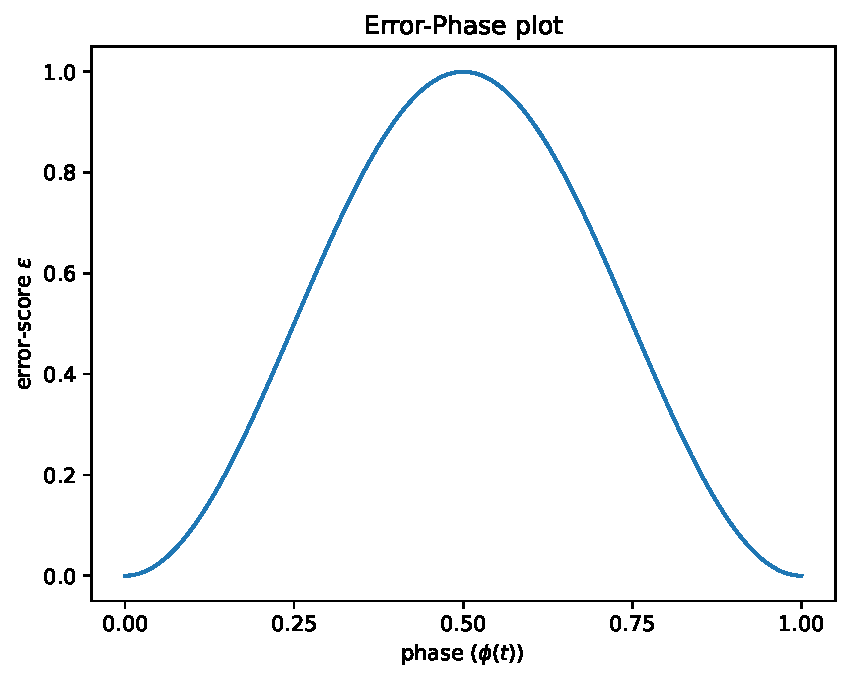
\includegraphics[width=0.8\linewidth]{Assets/Figures/PhaseErrorFunction.pdf}
		\caption{Error Measurement \eqref{error_measurement} plotted as a function of Phase}
		\label{fig:error_measurement}
	\end{figure}
	
	As we can see from this Error-Function, the error-score is close to 0 when the agent's phase $\phi_i(t)$ is itself close to 0 or 1 (i.e. the agent either just fired/flashed, or is about to fire/flash very soon). The error-score is the largest when an agent perceives a ``fire''-signal while being half-way through its own phase (i.e. having phase $\phi(t)=0.5$). We could also then ask ourselves, does not this go against the main/target goal of the system, being \textit{harmonic synchrony} — if agents are allowed to be ``half as fast'' as each other? 
	
	\lab{Hypotetisk scenario}{
		We could imagine a completely ``legal'' and harmonically synchronous scenario where two agents have half and double the frequency of each other. The agent with half the frequency of the faster agent would then have phase $\phi(t)=0.5$ when it would hear the faster agent ``fire''/``flash'' — leading to its Error-score $\epsilon(0.5) = sin^2(\pi/2) = 1$, which then makes it seem like the slower agent is maximally out of synch, when it is actually perfectly and harmonically synchronized. This calls out for an attenuating mechanism in our frequency update function, in order to ``cancel out'' this contribution so that perfectly harmonically synchronized agents will not be adjusted further despite their high Error-measurement.
	}
	
	This Error-Measurement/-Score forms the basis and fundament for the first component of Self-awareness, being the \textit{self-assessed synchrony-score} $s(n)$.
	
	% Om s(n):
	\subsubsection{Step 2: The first self-awareness component, s(n)}
	This aforementioned self-assessed synchrony-score, $s(n)$, is in fact simply the median of a list containing \textit{m} Error-scores $\epsilon$. Such a list is easily implemented in C\# by declaring a List$<$float$>$ called \textit{errorBuffer} e.g. (i.e. \textit{errorBuffer} is a list containing floating point values):
	
	\begin{equation}
	\label{error_buffer}
		errorBuffer = \{\epsilon(n), \epsilon(n-1), ... , \epsilon(n-m)\},
	\end{equation} \nl
	
	then leading to:
	
	\begin{equation}
	\label{self_assessed_synch}
		\begin{array}{rrclcl}
		s(n) & = & median(errorBuffer) \\ 
		& = & median(\{\epsilon(n), \epsilon(n-1), ... , \epsilon(n-m)\}) \in [0, 1],
		\end{array}
	\end{equation} \nl
	
	where $n$ is the latest observed ``fire-event'', and $m$ is the number of the last observed ``fire''-events we would like to take into account when calculating the self-assessed synch-score.
	
	If we then have a high $s(n)$-score, it tells us that the median of the $k$ last error-scores is high, or in other words that we have mainly high error-scores — indicating that this agent is out of synch. Conversely, if we have a low $s(n)$-score, indicating mainly low error-scores for the agent — then we have an indication that the agent is in synch, hence leading to low error scores, and in turn low $s(n)$-scores. 
	
	In other words, each agent hence has a way to assess themselves in how much in- or out-of-synch they believe they are compared to the rest of the agents. This is then the first degree/aspect of \opphoy{public} self-awareness in the design.
	
	% Om rho(n):
	\subsubsection{Step 3: frequency update amplitude- \& sign-factor, $\rho(n)$}
	
	Describing the amplitude and sign of the frequency-modification of the n-th ``fire-event'' received. It is used to say something about in which direction, and in how much, the frequency should be adjusted.
	
	\begin{equation}
	\label{amp_sign_freq_adj}
		\rho(\phi) = - sin(2\pi\phi(t)) \in [-1, 1]
	\end{equation}
	
	For example, if an agent $i$ has phase $\phi_i(t)=1/4$, it gets a value $\rho(1/4) = - sin(\pi/2) = -1$; meaning, the agent's frequency should be decreased (with the highest amplitude actually) in order to "slow down" to wait for the other nodes. Conversely, if an agent $j$ has phase $\phi_j(t)=3/4$, it gets a value $\rho(3/4) = - sin(3/2 \pi) = -(-1) = 1$; meaning, the agent's frequency should be increased (with the highest amplitude) in order to getting "pushed forward" to catch up with the other nodes.
	
	Acts as an attenuating factor, when $\phi(t)\approx0.5$, in the making of the H-value — supporting the goal of \textit{harmonic synchrony}.

	% Om H(n)-verdiene:
	\subsubsection{Step 4: the H-value, and the H(n)-list}
	
	The following value, being ``frequency-update-contributions'', is then (as previously mentioned) calculated immediately when the agent perceives another agent's ``flashing''-signal:
	
	\begin{equation}
	\label{h_value}
		H(n) = \rho(n) \cdot s(n)
	\end{equation}
	
	Here we then multiply a factor $\rho(n)$ representing how much, as well as in which direction, the agent should adjust its frequency, together with a factor $s(n) \in [0,1]$ of the adjusting agent's self-assessed synch-score. To recall, the self-assessed synch-score $s(n)$ tells an adjusting agent how in- or out-of-synch it was during the last $m$ perceived ``fire''-/``flash''-events — where $s(n)=0$ signifies a mean of 0 in error-scores, and $s(n)=1$ signifies a mean of 1 in error-scores. So then if this $H$-value is to be used to adjust the nodes's frequencies with, the frequency will then be adjusted in a certain direction and amount (specified by $\rho(n)$) — given that the agent is \textit{enough} ``out of synch''/``unsynchronized'' (in the case $s(n)$ is considerably larger than 0).
	
	The H-value says something about how much ``out of phase'' the agent was at the time the agent's $n$th ``flashing''-signal was perceived (and then followingly how much it should be adjusted, as well as in which direction after having been multiplied together with a sign-factor $\rho(n))$, given then that this H-value also consists of the \textit{self-assessed synch score s(n)} — which again simply was the median of the list of error-scores, \textit{errorBuffer} in our case.
	
	We could look at this $H$-value as representing the direction and amplitude of the frequency adjustment weighted by the need to adjust (due to being out of synch) at the time of hearing ``fire''-/``flash''-event $n$. Or in other words, this $H$-value is then the $n$-th contribution with which we want to adjust our frequency with.
	
	Especially interesting cases are when we have $\phi(n)\approx0.5 \implies \rho(n)\approx\pm0$, as well as the last $m$ Error-scores $\epsilon(n)$ being close to 0, also leading to $s(n)\approx0$. In both of these two cases the entire frequency-adjustment contribution $H$ would be cancelled out, due to harmonic synchronization (legally hearing a ``fire''-/``flash''-event half-way through ones own phase) in the first case, and due to not being out of synch in the latter (having low Error-Measurements). Cancelling out the frequency adjustment contribution in these cases is then not something bad, but something wanted and something that makes sense. If these $H$-values then are cancelled out or very small, it is indicative of that nodes are already in \textit{harmonic synchrony}, and hence should not be ``adjusted away'' from this goal state. On the other side, if these $H$-values then are different (e.g. closer to -1 and 1), it is indicative of that nodes are not yet in \textit{harmonic synchrony}, and that they hence should be ``adjusted closer'' to the goal state.
	
	All the calculated H-values are in my implementation accumulated and stored in an initially empty C\#-list (of floats), referred to as $H(n)$, at once they are calculated. The $H(n)$-list is then consecutively ``cleared out'' or ``flushed'' when its H-values have been used for the current cycle/period's frequency adjustment (i.e. at the phase climax, when $\phi(t)=1$), and is then ready to accumulate new H-values during the next cycle/period.
	
	% Om F(n) og selve oppdateringen av frekvens:
	\subsubsection{The final step: the frequency update function, $\omega_i(t^+)$}
	
	Now, we can pull it all together, for Nymoen et al.'s Frequency Adjustment approach for achieving harmonic synchrony with initially randomized and heterogenous frequencies.
	
	When an agent $i$ has a phase-climax ($\phi_i(t)=1$), it will update/adjust its frequency to the new $\omega_i(t^+)$ accordingly:
	
	\begin{equation}
	\label{freq_adj}
		\omega_i(t^+) = \omega_i(t) \cdot 2^{F(n)},
	\end{equation}
	
	where $t^+$ denotes the time-step immediately after phase-climax, and $F(n)$ is found by:
	
	\begin{equation}
	\label{f_value}
		F(n) = \beta\sum_{x=0}^{k-1}\frac{H(n-k)}{k},
	\end{equation}
	
	where $\beta$ is the frequency coupling constant, $k$ is the number of heard/received ``fire-event''s from the start of the last cycle/period to the end (i.e. the phase-climax, or \textit{now}) — and the rest of the values are as described above.
	
	This $F(n)$-value then, as we see in Equation \eqref{f_value}, is a weighted average of all the agent's $H(n)$-values accumulated throughout the agent's last cycle.
	
	
	
	
	
	% FREQ.-SYNCH APPROACH 3: HIGH LEVEL Self-Awareness
	% Hopefully an improved method with some additional Self-Awareness components
	\subsection{Thorvaldsen's high SA-leveled frequency-adjustment}
	
	\gjor{Beskriv min nye proposede algoritme (to-be-implemented) for å oppnå harmonisk synkronitet i $\phi$- \& $\omega$-problemet med frequency-adjustment, som inneholder flere tilleggs- Self-Awareness-komponenter, sammenliknet med K. Nymoens frequency-adjustment metode. Eksempler på slike tilleggs- Self-Awareness-komponenter er såkalt Belief-awareness (som fanger usikkerhet og tillits-nivåer) og/eller Expectation-awareness (som kombinerer Belief-awareness og Time-awareness) \cite{sacs17_ch3}. Andre forslag er å implementere Self-Awareness i forhold til, og vekte frekvensoppdaterings-bidragene H(n) i henhold til:
	\begin{itemize}
		\item avstand: f.eks. $H^*(n)= H(n) \cdot \frac{1}{distance}$ for ``fire''-event $n$, så lenge ikke $distance = 0$.
		\item hvem som er hvem (i.e. agent\_id).
		\item større median-liste ift. den self-assessed'e synch-score'n $s(n)$ og $errorBuffer$'et. Dette kan være nyttig ved større collective-sizes, da et lite/kort median-filter/-$errorBuffer$-liste vil kunne miste eller gå glipp av error-scores, $\epsilon(n)$, fra ``fire''-events fra langt tilbake (tidlig) i ``oppsamlings-perioden.''
		\item de andres frekvenser. Høre etter og registrere andre individers ``fire''-signaler kontinuerlig og estimere disse individenes frekvenser utifra det (f.eks. $\hat{\omega}_j = time_{j, fired\_now} - time_{j, fired\_last\_time}$, eller et gjennomsnitt av slike oppsamlede verdier).
	\end{itemize}
	}





% SECTION 4, Om target-staten til systemet: harmonic synchrony
\section{System target state: harmonic synchrony}
\label{sec:harmonic_synchrony}

As previously mentioned, this state of \textit{harmonic synchrony} is then the system goal state which we want the musical robot-collective to end up in eventually, and the sooner the better.

The state of harmonic synchrony is defined as the state in which all agents in the musical collective ``fire''/``flash'', as described in Subsection \ref{subsec:fire_signal}, at an even underlying interval or pulse, a certain number of times in a row. This is not to say all agents will have to ``fire''/``flash'' simultaneously, as has traditionally been the case for pulse-coupled oscillators \cite{}.

So for phases to be harmonically synchronized, they have to be so that they climax ..................

As one is creating an interactive music technology system, one might want to encourage and allow for the playing of various musical instruments at various rhythms/paces, as it might be quite boring if all instruments were played at the exact same measure or pulse. As K. Nymoen et al. \cite{nymoen_synch} reason when discussing their own interactive ``Firefly'' music-system, as well as coining the term of harmonic synchrony: \nl

``\textit{Temporal components in music tend to appear in an integer-ratio relation to each other (e.g., beats, measures, phrases, or quarter notes, 8ths, 16ths)}.'' \nl

and \nl

``\textit{Being an interactive music system, people may want their device to synchronize with different subdivisions of a measure (e.g. some play quarter notes while others play 8ths).}'' \nl

Accomodating for these aspects then, K. Nymoen et al. \cite{nymoen_synch} took inspiration for achieving synchronization in a decentralized system from the concept of \textit{harmonics} in the frequency spectrum of a waveform, in that each harmonic wave or overtone has a frequency with an integer-relationship to the fundamental (smallest) frequency. This phenomenon can e.g. be seen in the frequency spectrogram of a humanly hummed G3-tone, in Figure \ref{fig:sub:G3_hummed_waveform}, where we can observe the harmonics and overtones having frequencies with integer relationships to the fundamental (smallest) frequency, which was meant to be 195,99 Hz.

% a waveform with a fundamental frequency of 195,99 Hz (i.e. a G3-note and $\approx$ 200 Hz) has harmonics and overtones with frequencies with integer relationships to said fundamental frequency.

\begin{figure}[ht!]
	\centering
		\begin{subfigure}[t]{.5\textwidth}
			\centering\captionsetup{width=.9\linewidth}%
			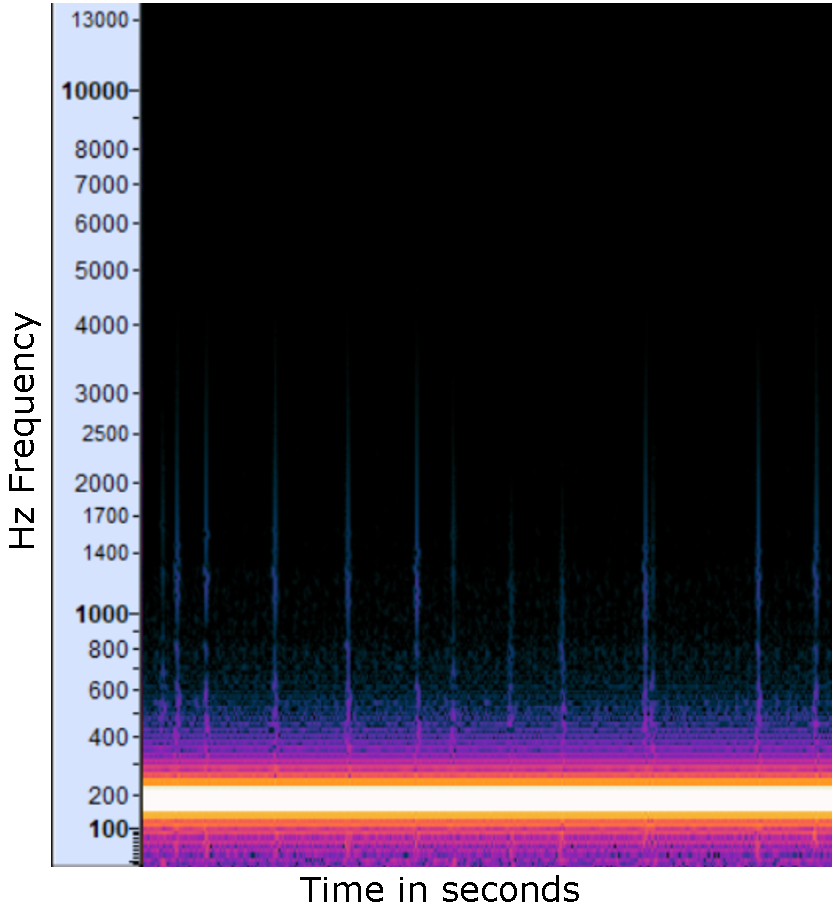
\includegraphics[width=0.9\linewidth]{Assets/Figures/G3_196Hz_PureTone_waveform_spectrogram.pdf}
			\caption{The frequency spectrogram of an audible waveform being a monotone and purely generated \cite{generate_tones} G3-tone at 195,99 Hz.}
			\label{fig:sub:G3_pure_waveform}
		\end{subfigure}%
		\begin{subfigure}[t]{.5\textwidth}
			\centering\captionsetup{width=.9\linewidth}%
			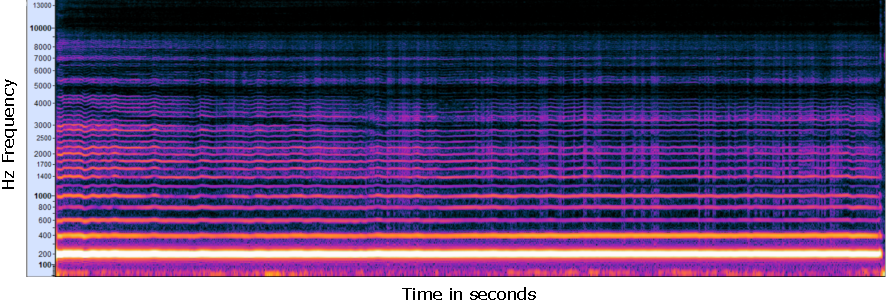
\includegraphics[width=0.9\linewidth]{Assets/Figures/G3_196Hz_HummingWaveform_FrequencySpectrum.pdf}
			\caption{The frequency spectrogram of an audible waveform being a more-or-less monotone but non-pure G3-tone, hummed and recorded by me \cite{}, according to what I perceived as the G3-tone when I heard the waveform corresponding to \ref{fig:sub:G3_pure_waveform} with my own ears.}
			\label{fig:sub:G3_hummed_waveform}
		\end{subfigure}
	\caption{Frequency spectrograms of two different-sounding waveforms of the same G3-tone at 195,99 Hz. Frequencies in a harmonically synchronized agent collective will for the first $\phi$-problem resemble the frequencies in \ref{fig:sub:G3_pure_waveform}, since all frequencies in this problem are equal and constant. Conversely, when frequencies can be heterogenous, as in the $\phi$- \& $\omega$-problem, the frequencies in a harmonically synchrnonized agent collective will resemble more the frequencies in \ref{fig:sub:G3_hummed_waveform}, where harmonics and overtones (i.e. frequencies in integer-relationships to the fundamental and lowest frequency) are present.}
	\label{fig:frequency_spectrograms}
\end{figure}



\inkl{This is exactly how the frequencies of the individual musical agents in our music-collective must be, in order for the agent-collective to be harmonically synchronized.

So for frequencies to be harmonically synchronized, they have to be so that ..................
}



More accurately then, all musical agents—in a harmonically synchronized state—will have frequencies $\in \omega_{0} \cdot 2^{\mathbb{N}_0}$, where $\omega_{0}$ is the agent with the lowest frequency's frequency (i.e. the fundamental frequency), and $\mathbb{N}_0$ is the mathematical set of natural numbers including the number zero. Hence, agents will typically have frequencies like $\omega_{0} \cdot 2^0 = \omega_{0}$, $\omega_{0} \cdot 2^1 = 2\omega_{0}$, $\omega_{0} \cdot 2^2 = 4\omega_{0}$, or $\omega_{0} \cdot 2^3 = 8\omega_{0}$. If all agents end up with these kind of frequencies, we say they have ``legal'' and harmonically synchronized frequencies.







% Presenting the Performance-measure used to evaluate the implemented methods (Benchmark?):
\section{Performance-measure: time until goal of harmonic synchrony is detected}
\label{sec:performance_measure}

Hvordan detektere harmonic synchrony. \nl

Hvordan HSYNCHTIME er definert. \nl

\textbf{Node-firing plot}.